\chapter{Gaussian Processes}
\label{chapter:gp}

This chapter describes the technical details of the Gaussian distribution and
its extension, the Gaussian Process (GP). We believe it is important to have at
least a basic understanding of the underlying math to make claims
about the behavior of the model, especially since GPs behave quite differently
than other parametric machine learning models.

Since our objective is Bayesian optimization, we only derive the properties
necessary for its implementation. Specifically, we are interested in the
conditional and marginal distributions of a multivariate Gaussian. The
conditional Gaussian distribution allows us to compute the posterior $p(f|x)$
at an arbitrary point, and the marginal allows us to fit a GP regression model
to each hyperparameter separately for additional visualization.

Let us now continue with a more rigorous treatment of the Gaussian distribution.
For a more thorough treatment, see \cite{bishop2016pattern} and \cite{murphy2012machine}.

\begin{defn}
  A random variable $\rX$ has a \newterm{univariate Gaussian distribution},
  written as $\rX \sim \mathcal{N}(\mu, \sigma^2)$, when its density is
  $$
    p(x) = \frac{1}{\sqrt{2\pi\sigma^2}} \exp{\left\{ -\frac{1}{2\sigma^2} (x - \mu)^2 \right\}}.
  $$
  The parameters $\mu$ and $\sigma$ are its \emph{mean} and \emph{standard deviation}.
\end{defn}

\begin{defn}
  We say that $\rX$ has a \newterm{degenerate Gaussian distribution} when $\rX \sim \mathcal{N}(\mu, 0)$, which formally becomes a Dirac delta function centered around $\mu$.
\end{defn}

% TODO: \mX vs \rX pro vicerozmerne rv
\begin{defn}
  A random variable $\mX \in \mathbb{R}^n$ has a \newterm{multivariate Gaussian distribution} if
  any linear combination of its components is a univariate Gaussian, i.e.
  $\va^T \rX = \mSigma_{i=1}^n \va_i \mX_i$ is a Gaussian for all $\va \in \mathrm{R}^n$.
  % TODO: cov sequence?
  We then write $\mX \sim \mathcal{N}(\vmu, \mSigma)$ where $\mathbb{E}[\mX_i] = \mu_i$
  and $cov(\mX_i, \mX_j) = \mSigma_{ij}$.
\end{defn}


\begin{rem}
  The parameters $\vmu$ and $\mSigma$ uniquely determine the distribution $\mathcal{N}(\vmu, \mSigma)$.
\end{rem}

\begin{defn}
  A random variable $\mX \sim \mathcal{N}(\vmu, \mSigma)$ has a \newterm{degenerate multivariate Gaussian distribution}
  if $\det \mSigma = \mZero$.
\end{defn}

\begin{rem}
  Given a random variable $\mX \sim \mathcal{N}(\vmu, \mSigma)$, random variables $\mX_1, \ldots,
  \mX_n$ are independent with distributions $\mX_i \sim \mathcal{N}(\mu_i, \sigma_i^2)$ if and only
  if $\vmu = (\mu_1, \ldots, \mu_n)$ and $\mSigma = diag(\sigma_1^2, \ldots, \sigma_n^2)$.
\end{rem}

\begin{thm}
  Given two random variables $\mX, \mY$ that are jointly Gaussian, they are independent if and only if $cov(\mX, \mY) = 0$. Note that
  this statement is not true for any random variable, and it is only a special property of the
  multivariate Gaussian.
\end{thm}

\begin{proof}
	Consider the case of only a two-dimensional random vector $\mX$ with a multivariate Gaussian distribution. When $\operatorname{cov}(\mX_1, \mX_2) = 0$ the covariance matrix $\mSigma$ is a diagonal matrix, and the density factorizes into a product of two marginal densities.
	
	In case $\mX$ and $\mY$ are jointly Gaussian random vectors which are uncorrelated, their covariance is a block diagonal matrix, which again trivially factors in two marginal densities.
\end{proof}

\begin{thm}
  A Gaussian random variable $\rX \sim \mathcal{N}(\vmu, \mSigma)$ has density if and only if
  it is non-degenerate (i.e.\ $\det \mSigma \neq 0$, alternatively $\mSigma$
  is positive-definite). In this case, the density is

  \begin{equation}
    \label{eq:mvn-definition}
    p(\vx) = \frac{1}{\sqrt{\det(2 \pi \mSigma)}} \exp{ \left\{ - \frac{1}{2}
    (\vx - \vmu)^T \mSigma^{-1} (\vx - \vmu) \right\} }.
  \end{equation}
\end{thm}

\begin{rem}
  The normalizing constant in the denominator is also often presented in an alternate
  form $$\det(2 \pi \mSigma) = (2\pi)^n \det(\mSigma),$$ which follows from basic
  determinant properties. Alternatively, we can also move the square root in the
  exponent and write $(2 \pi)^{n/2} (\det \mSigma)^{1/2}$.
\end{rem}

\begin{rem}
  In a special case of the multivariate Gaussian with $n = 1$, we have
  $\mSigma = \sigma^2$ (meaning $cov(X, X) = \sigma^2$) and $\mSigma^{-1} =
  \frac{1}{\sigma^2}$, and hence the multivariate Gaussian formula becomes
  a univariate one:

  \begin{equation}
    p(x) = \frac{1}{\sqrt{2 \pi \sigma^2}} \exp{\left\{ - \frac{1}{2\sigma^2} (x - \mu)^2 \right\}}.
  \end{equation}
\end{rem}

\section{Sampling}

Even not of immediate interest for Bayesian optimization, we shortly show
how to generate samples from a multivariate Gaussian, because the ability is useful for
visualization purposes with GPs.

\begin{thm}
  Given a random variable $\mX$ with $cov[\mX] = \mSigma$, it follows from
  the definition of covariance that $cov[\mA \mX] = \mA \mSigma \mA^T$.
\end{thm}

\begin{proof}
  \begin{align}
    cov[\mA \mX] &= E[(\mA \mX - E[\mA \mX])(\mA \mX - E[\mA \mX])^T] \\
                 &= E[(\mA \mX - \mA E[\mX])(\mA \mX - \mA E[\mX])^T] \\
                 &= E[\mA (\mX - E[\mX])(\mX - E[\mX])^T \mA^T] \\
                 &= \mA E[(\mX - E[\mX])(\mX - E[\mX])^T] \mA^T \\
                 &= \mA cov[\mX] \mA^T \\
                 &= \mA \mSigma \mA^T
    \label{eq:gaussian-ax}
  \end{align}
\end{proof}

\begin{thm}
  Given a random variable $\mX \sim \gN(\mZero, \mI)$ and a positive-definite matrix
  $\mSigma$ with a Cholesky decomposition $\mSigma = \mL \mL^T$, then

  \begin{equation}
    \mL \mX \sim \gN(\mZero, \mSigma).
    \label{eq:gaussian-cholesky}
  \end{equation}
\end{thm}

\begin{proof}
  We can immediately use \autoref{eq:gaussian-ax}.
  \begin{align}
    \mL \mX \sim N(\mZero, \mL \mI \mL^T) = N(\mZero, \mL \mL^T) = N(\mZero, \mSigma).
  \end{align}
\end{proof}

\begin{thm}
  Any affine transformation of a Gaussian is a Gaussian. In particular,
  $$
    \rX \sim \gN(\vmu, \mSigma) \implies \mA \rX + \vb \sim \gN(\mA \vmu + \vb, \mA \mSigma \mA^T)
  $$
  for any $\vmu \in \mR^n, \mSigma \in \mR^{n \times n}$ positive
  semi-definite, and any $\mA \in \mR^{m \times n}, \vb \in \mR^m$.
  We call this the \newterm{affine property} of a Gaussian.
\end{thm}

\begin{proof}
  Follows from the linearity of expectation together with \autoref{eq:gaussian-cholesky}.
\end{proof}

Since samples from $\gN(\mZero, \mI)$ can be generated easily, using the
affine property we can generate samples from an arbitrary multivariate
Gaussian. All that is required is a procedure for Cholesky decomposition, and a
way of generating independent samples from a univariate Gaussian, which can be
achieved using the Box-Muller transform \citep{box-muller1958note}.


\section{Geometric Properties}

If $\mSigma$ is positive-definite, then $\mY \sim \gN(\vmu, \mSigma)$ implies
$\mA^{-1} (\mY - \vmu) \sim \mathcal{N}(\mZero, \mI)$ where $\mSigma = \mA \mA^T$.  The random
variable $\mA^{-1} (\mY - \vmu)$ has a spherical shape in $n$-dimensional
space.

Looking further at the density formula for a multivariate Gaussian
(\autoref{eq:mvn-definition}), the term $(\vx - \vmu)^T \mSigma^{-1}(\vx -
\vmu)$ is called the Mahalanobis distance between $\vx$ and $\vmu$. If we
consider $\vmu$ a constant, we can also view it as a quadratic form in $\vx$.
When $\mSigma$ is an identity matrix, the Mahalanobis distance reduces to
Euclidean distance. In general, it can be thought of as a distance on a
hyper-ellipsoid. Let us now derive some intuition for that.

Since $\mSigma$ is a covariance matrix, we know it is positive definite, and we
can perform its eigendecomposition to get $\mSigma = \mU \mLambda \mU^T$, where
$\mU$ is an orthogonal matrix of eigenvectors, and $\mLambda$ is a diagonal
matrix of eigenvalues. Basic matrix algebra gives us
$$
  \mSigma^{-1} = (\mU^T)^{-1} \mLambda^{-1} \mU^{-1} = \mU \mLambda^{-1}
  \mU^T = \sum_{i = 1}^D \frac{1}{\lambda_i} \vu_i \vu_i^T,
$$
where the second to last equality comes from $\mU$ being orthogonal ($\mU^{-1}
= \mU^T$).  Substituting this in the Mahalanobis distance we get
\begin{align}
  (\vx - \vmu)^T \mSigma^{-1} (\vx - \vmu) &= (\vx - \vmu)^T \left( \sum_{i = 1}^D \frac{1}{\lambda_i} \vu_i \vu_i^T \right) (\vx - \vmu) \\
                                           &= \sum_{i = 1}^D (\vx - \vmu)^T \frac{1}{\lambda_i} \vu_i \vu_i^T (\vx - \vmu) \\
                                           &= \sum_{i = 1}^D \frac{y_i^2}{\lambda_i}, \label{eq:mvn-ellipse}
\end{align}
where $y_i = u_i^T (\vx - \vmu)$ has exactly the same form as a $D$-dimensional
ellipse. From this we conclude that the contour lines of a
multivariate Gaussian will be elliptical, where the eigenvectors determine the
orientation of the ellipse, and the eigenvalues determine the length of the
principal axes \citep{bishop2016pattern}.



\section{Conditional and Marginal Gaussian Distribution}

In this section we derive the conditional $p(x_1 | x_2)$ and marginal $p(x_1)$
for a given joint distribution $p(x_1, x_2)$. One of the interesting properties
of a multivariate Gaussian is that both the conditional and the marginal are
also Gaussian, and we can easily compute their parameters in closed from based
on the parameters of the joint distribution.

Before we derive the conditional and marginal distributions, let us state
the partitioned inverse formula without a proof.

\begin{thm}[\citep{murphy2012machine}] Consider a partitioned matrix

  \begin{equation}
    \mM = \begin{bmatrix} \mE & \mF \\ \mG & \mH \end{bmatrix}
  \end{equation}

  where we assume $\mE$ and $\mH$ are invertible. Then

  \begin{align}
    \mM^{-1} &= \begin{bmatrix}
      (\mM / \mH)^{-1} & -(\mM / \mH)^{-1} \mF \mH^{-1} \\
      -\mH^{-1} \mG (\mM \mH)^{-1} & \mH^{-1} + \mH^{-1} \mG (\mM / \mH)^{-1} \mF \mH^{-1}
    \end{bmatrix} \\
             &= \begin{bmatrix}
      \mE^{-1} + \mE^{-1} \mF (\mM / \mE)^{-1} \mG \mE^{-1} & - \mE^{-1} \mF (\mM / \mE)^{-1} \\
      -(\mM / \mE)^{-1} \mG \mE^{-1} & (\mM / \mE)^{-1}
    \end{bmatrix},
    \label{eq:matrix-inversion-lemma}
  \end{align}

  where

  \begin{align}
    \mM / \mH &= \mE - \mF \mH^{-1} \mG \\
    \mM / \mE &= \mH - \mG \mE^{-1} \mF
  \end{align}

  is called the \newterm{Schur complement}.
\end{thm}

\begin{proof}
  Since the proof is rather technical and only consists of applying the
  LDU decomposition and many algebraic manipulations, we leave it out and
  refer the reader to \cite{murphy2012machine} for details.
\end{proof}


\subsection{Conditional Distribution is a Gaussian}

Suppose $\vx$ is a $D$-dimensional random vector with a multivariate Gaussian distribution
$\gN(\vx | \vmu, \mSigma)$, and that $\vx$ is partitioned into two vectors
$\vx_1$ and $\vx_2$ such that

\begin{equation}
  \vx = \partx
\end{equation}

We also partition the mean vector $\vmu$ and the covariance matrix $\mSigma$
into a block matrix, and name the inverse of the covariance matrix $\mLambda =
\mSigma^{-1}$, which simplifies a few of the equations that follow. We
derive the exact form of $\mLambda$ and of its individual blocks later in this
section. For now we simply use the fact that $\mSigma$ is positive-definite,
and thus it is invertible. The matrix $\mLambda$ is also known as a
\newterm{precision matrix}.

\begin{equation}
  \vmu = \partmu,
  \mSigma = \partsigma, \mLambda = \mSigma^{-1} = \partlambda \label{eq:mvn-partition}
\end{equation}

Note that since $\mSigma$ is a symmetric matrix, $\ms{12}^T = \ms{21}$, and
similarly $\ml{12}^T = \ml{21}$. Similarly, $\ms{11}$, $\ms{22}$, $\ml{11}$,
and $\ml{22}$ are all symmetrical.

Before we derive the parameters of the conditional, we show that the
conditional distribution $p(x_1 | x_2)$ is a Gaussian. To do this, we take the
joint distribution $p(x_1, x_2)$ and fix the value of $x_2$
\citep{bishop2016pattern}. Using the definition of the conditional probability
$p(x_1, x_2) = p(x_1 | x_2) p(x_2)$ we can see that after fixing the value of
$x_2$, $p(x_2)$ is simply a normalization constant, and the remaining term
$p(x_1 | x_2)$ is a function of $x_1$ which together with the normalization
constant gives us the conditional probability distribution on $x_1$.
We now use the partitioned form of the multivariate Gaussian defined by
\autoref{eq:mvn-partition} to show that $p(x_1 | x_2)$ is actually a Gaussian.

Let us begin by looking at the exponent in \autoref{eq:mvn-definition}:

\begin{align}
  -\frac{1}{2} (\vx - \vmu)^T \mLambda (\vx - \vmu) &=
  -\frac{1}{2} \left(\partx - \partmu \right)^T \partlambda \left(\partx - \partmu \right) \\
                                                    &= -\frac{1}{2} \partxmu^T \partlambda \partxmu
\end{align}

To make the next few equations easier to follow we set $\vy_1 = \vx_1 - \vmu_1$ and $\vy_2 = \vx_2 - \vmu_2$.

\begin{align}
    -\frac{1}{2} \begin{bmatrix} \vy_1 \\ \vy_2 \end{bmatrix} ^T & \partlambda \begin{bmatrix} \vy_1 \\ \vy_2 \end{bmatrix} = \\
  %
  \begin{split}
    ={}& -\frac{1}{2} \begin{bmatrix} \vy_1 \ml{11} + \vy_2 \ml{21} \\ \vy_1 \ml{12} + \vy_2 \ml{22} \end{bmatrix} ^T \begin{bmatrix} \vy_1 \\ \vy_2 \end{bmatrix}
  \end{split} \\
  %
  \begin{split}
    ={}& -\frac{1}{2} \left( \vy_1^T \ml{11} \vy_1 + \vy_2^T \ml{21} \vy_1 + \vy_1^T \ml{12} \vy_2 + \vy_2^T \ml{22} \vy_2 \right)
  \end{split} \\
  %
  \begin{split}
    ={}& -\frac{1}{2} (\vx_1 - \vmu_1)^T \ml{11} (\vx_1 - \vmu_1) {}+ \\
       &-\frac{1}{2} (\vx_2 - \vmu_2)^T \ml{21} (\vx_1 - \vmu_1) {}+ \\
       &-\frac{1}{2} (\vx_1 - \vmu_1)^T \ml{12} (\vx_2 - \vmu_2) {}+ \\
       &-\frac{1}{2} (\vx_2 - \vmu_2)^T \ml{22} (\vx_2 - \vmu_2) \label{eq:mvn-quadratic-form}
  \end{split}
\end{align}

We see that this is a quadratic form in $x_1$, and hence the corresponding
conditional distribution $p(x_1 | x_2)$ is a Gaussian. 
Because the Gaussian distribution is completely defined by its mean and
covariance, we do not need to figure out the value of the normalization
constant. We simply have to derive the equations for $\vmu$ and $\mSigma$.

% Because we know $p(x_1, x_2) = p(x_1|x_2)p(x_2)$ and that both $p(x_1, x_2)$ and $p(x_1|x_2)$ are multivariate Gaussians, fixing the value of $x_1$ means that $p(x_1|x_2)$ as a function of $x_2$ is just a normalization constant, and $p(x_2)$ must have the same form as $p(x_1, x_2)$ and therefore is also a multivariate Gaussian. \todo{tady ten marginal nevim jiste}

% TODO: x2 je spatne (marignal)



%	At this point we know that the joint distribution factors into two multivariate
%	Gaussians, that is
%	\begin{align}
%	p(x_1, x_2) &= p(x_1 | x_2) p(x_2) \\
%	&= \gN(x_1 | \vmu_{1|2}, \ms{1|2}) \gN(x_2 | \vmu_2, \ms{22})
%	\end{align}
%	and we only need to infer their parameters.

We continue with the proof from \cite{murphy2012machine}. We will make use of
the partitioned matrix inverse theorem \autoref{eq:matrix-inversion-lemma}.
To make the equations more
readable, we again define
\begin{align}
    \vy_1 &= \vx_1 - \vmu_1 \\
    \vy_2 &= \vx_2 - \vmu_2.
\end{align}
We then simply take the block definition of a multivariate Gaussian and
multiply everything out

{\setlength{\arraycolsep}{5pt}
  \begin{align}
      \llap{E} &= \exp \left\lbrace -\frac{1}{2}
      \begin{bmatrix} \vy_1 \\ \vy_2 \end{bmatrix}^T
      \partsigma
      \begin{bmatrix} \vy_1 \\ \vy_2 \end{bmatrix} \right\rbrace \\
      %
      &= \exp \left\lbrace -\frac{1}{2}
      \begin{bmatrix} \vy_1 \\ \vy_2 \end{bmatrix}^T
      \begin{bmatrix} \mI & \mZero \\ -\mSigma_{22}^{-1} \mSigma_{21} & \mI \end{bmatrix}
      \begin{bmatrix} (\mSigma/\mSigma_{22})^{-1} & \mZero \\ \mZero & \mSigma_{22}^{-1} \end{bmatrix}
      \begin{bmatrix} \mI & -\mSigma_{12} \mSigma_{22}^{-1} \\ \mZero & \mI \end{bmatrix}
      \begin{bmatrix} \vy_1 \\ \vy_2 \end{bmatrix} \right\rbrace \\
      %
      &= \exp \left\lbrace -\frac{1}{2}
      \begin{bmatrix} \vy_1^T - \vy_2^T (\mSigma_{22}^{-1} \mSigma_{21}) \\
      \vy_2
      \end{bmatrix}^T
      \begin{bmatrix} (\mSigma/\mSigma_{22})^{-1} & \mZero \\ \mZero & \mSigma_{22}^{-1} \end{bmatrix} \begin{bmatrix} \vy_1 -\mSigma_{12} \mSigma_{22}^{-1} (\vy_2) \\ \vy_2 \end{bmatrix} \right\rbrace \\
      %
      &= \exp \left\lbrace -\frac{1}{2}
      \begin{bmatrix} (\vy_1^T - \vy_2^T \mSigma_{22}^{-1} \mSigma_{21}) (\mSigma/\mSigma_{22})^{-1} \\
      \vy_2^T \mSigma_{22}^{-1}
      \end{bmatrix}^T
      \begin{bmatrix} \vy_1 -\mSigma_{12} \mSigma_{22}^{-1} (\vy_2) \\ \vy_2 \end{bmatrix}
      \right\rbrace \\
      %
      &= \exp \left\lbrace -\frac{1}{2}
      (\vy_1^T - \vy_2^T \mSigma_{22}^{-1} \mSigma_{21}) (\mSigma/\mSigma_{22})^{-1} (\vy_1 -\mSigma_{12} \mSigma_{22}^{-1} \vy_2)
      \right\rbrace \times
      \label{eq:mvn-two-quadratic-forms}
      \\
      & \qquad\qquad \times \exp \left\lbrace -\frac{1}{2} \vy_2^T \mSigma_{22}^{-1} \vy_2 \right\rbrace \nonumber
  \end{align}
}

We can immediately see that the first term is a quadratic form in $\vx_1$ when $\vx_2$ is held constant, and the second term is simply a normalization constant.
Let us now consider the
first term in isolation and move the terms around a little bit. We also make
use of the fact that because $\mSigma_{22}$ is a positive-definite matrix, its
inverse is also symmetric, so $\mSigma^{-1^T}_{22} = \mSigma^{-1}_{22}$. We
also know that $\mSigma^T_{12} = \mSigma_{21}$.

\begin{align}
    E_{1|2} &= \exp \left\lbrace -\frac{1}{2}
    (\vy_1^T - \vy_2^T \mSigma_{22}^{-1} \mSigma_{21}) (\mSigma/\mSigma_{22})^{-1} (\vy_1 -\mSigma_{12} \mSigma_{22}^{-1} \vy_2) \right\rbrace \\
    &= \exp \left\lbrace -\frac{1}{2}
    (\vy_1 - \mSigma_{12}\mSigma_{22}^{-1} \vy_2)^T (\mSigma/\mSigma_{22})^{-1} (\vy_1 -\mSigma_{12} \mSigma_{22}^{-1} \vy_2) \right\rbrace \\
    &= \exp \{ -\frac{1}{2}
    (\vx_1 - \vmu_1 - \mSigma_{12}\mSigma_{22}^{-1} (\vx_2 - \vmu_2)^T (\mSigma/\mSigma_{22})^{-1} \\
    & \hspace{40pt} (\vx_1 - \vmu_1 -\mSigma_{12} \mSigma_{22}^{-1} (\vx_2 - \vmu_2)) \}
    \label{eq:mvn-quadratic-form-12}
\end{align}

In \autoref{eq:mvn-quadratic-form-12} we observe a multivariate Gaussian density with
parameters
\begin{align}
  \vmu_{1|2} &= \vmu_1 + \mSigma_{12}\mSigma_{22}^{-1} (\vx_2 - \vmu_2) \\
  \mSigma_{1|2} &= (\mSigma/\mSigma_{22})^{-1} =  \ms{11} - \ms{12} \mSigma_{22}^{-1} \ms{21}.
  \label{eq:mvn-conditional-parameters}
\end{align}
At this point we know that $p(\vx_1, \vx_2) = c \cdot \mathcal{N}(\vmu_{1|2}, \mSigma_{1|2})$, where $c$ is some normalization constant. Here we make use of a general property of probability distributions, which tells us that the exponentiated quadratic form we obtained in \autoref{eq:mvn-quadratic-form-12} is the conditional Gaussian we are looking for, and not some other density. Because its value is finite and non-negative for all $\vx_1$, we can normalize it to a density by dividing \autoref{eq:mvn-quadratic-form-12} by its integral over $\mathrm{R}$. We do not even need to prove the existence of the integral, because in this particular case its value is exactly the normalization constant of a multivariate Gaussian.

The formula in \autoref{eq:mvn-conditional-parameters} is extremely important for the use of GPs as a probabilistic
model in Bayesian optimization. It allows us to compute the exact
parameters of the posterior $p(f|x)$ at any given point, and as a result
to compute the acquisition function.

\subsection{Marginal Distribution is a Gaussian}

Now that we know that $p(\vx_1 | \vx_2) \sim \mathcal{N}(\vmu_{1|2}, \mSigma_{1|2})$ we can again look at the quadratic forms in \autoref{eq:mvn-two-quadratic-forms}. Matching the left term to $\mathcal{N}(\vmu_{1|2}, \mSigma_{1|2})$ up to the normalization constant we are left with only
$$
\exp \left\lbrace -\frac{1}{2} \vy_2^T \mSigma_{22}^{-1} \vy_2 \right\rbrace.
\label{eq:mvn-marginal-exp}
$$
Together with the definition of conditional probability $p(\vx_1, \vx_2) = p(\vx_1 | \vx_2) p(\vx_2)$, and the fact that both $p(\vx_1, \vx_2)$ and $p(\vx_1 | \vx_2)$ are multivariate Gaussians, we conclude that $p(\vx_2)$ must also be a multivariate Gaussian, using the same argument with a density being defined up to a normalization constant.
The quadratic form in \autoref{eq:mvn-marginal-exp} immediately tells us the parameters of $p(\vx_2)$, specifically
$$
	p(\vx_2) \sim \mathcal{N}(\vmu_2, \mSigma_2).
	\label{eq:mvn-marginal-parameters}
$$
Intuitively, the marginal distribution of a multivariate Gaussian is obtained by simply ignoring all of the dimensions over which we are marginalizing, and only considering the parameters we are interested in.


\section{Gaussian Processes}

\newterm{Gaussian Process} is a stochastic process (a collection of random
variables), such that every subset of those random variables has a
multivariate Gaussian distribution. It is defined by a mean function
$m(\vx)$ and a covariance function $\kappa(\vx, \vx')$. Formally, we write
\begin{equation}
  p(\vx) \sim \mathcal{G}\mathcal{P} (m(\vx), \kappa(\vx, \vx')).
\end{equation}
Any finite subset $\vx = (x_1, \ldots, x_n)$ is jointly Gaussian with mean vector
$m(\vx)$ and covariance matrix $\mSigma(\vx)$, where $\mSigma(\vx)_{ij} =
\kappa(\vx_i, \vx_j)$, with $\kappa$ being any positive definite kernel
function \citep{murphy2012machine}.

The GP defines a prior distribution over functions $f$, which when
combined with data $x$ can be converted into a posterior distribution
over functions $p(f|x)$.

\subsection{GP Regression with Noise-free Observations}

Consider the case when we are predicting a function $f$
based on a few observations $\mathcal{D} = \{(\vx_1, y_1), \ldots, (\vx_n, y_n)\}$,
and we are interested in predicting the value of $y_\star = f(x_\star)$ at a new point
$x_\star$.

Using the definition of a GP, we know that all $y_i$ and $y_\star$ are jointly
Gaussian. Furthermore, these are the only points we are interested
in.  Even though the GP is a distribution over functions, that is over
infinitely dimensional vectors, we only need to consider finitely many
points and we can ignore the rest.  This is a crucial property of a GP and
essentially makes everything we are interested in performing possible.

By assuming a GP, we get all of the properties of a multivariate Gaussian
automatically, including a closed form solution to the conditional and marginal
distribution parameters. Let us now write the joint distribution of $\vy$ and $\vy_\star$ in
a partitioned form
$$
\begin{pmatrix} \vy \\ \vy_\star \end{pmatrix} \sim \mathcal{N}\begin{pmatrix}
  \begin{pmatrix} \vmu \\ \vmu_\star \end{pmatrix},
  \begin{pmatrix} \mK & \mK_\star \\ \mK_\star^T & \mK_{\star\star} \end{pmatrix}
  \end{pmatrix}
$$
where $\mK = \kappa(\mX, \mX)$, $\mK_\star = \kappa(\mX, \mX_\star)$, and
$\mK_{\star\star} = \kappa(\mX_\star, \mX_\star)$ \citep{williams2006gaussian}.
Note that $\vy$ and $\vy_\star$ can be either single points or
vectors, as we might be interested in computing the posterior over multiple
points at once given an existing dataset.  Because the posterior is just a multivariate
Gaussian, we can make use of the conditioning formula and compute the posterior
$p(\vy_\star | \mX_\star, \mX, \vy)$ exactly as
\begin{align}
  p(\vy_\star | \mX_\star, \mX, \vy) &= \mathcal{N}(\vy_\star | \vmu_\star, \mSigma_\star)
  \\
  \vmu_\star &= \vmu(\mX_\star) + \mK_\star^T \mK^{-1} (\vy - \vmu(\mX))
  \\
  \mSigma_\star &= \mK_{\star\star} - \mK_\star^T \mK^{-1} \mK_\star,
\end{align}
where $\vmu_\star$ is the mean and $\mSigma_\star$ is the covariance of the multivariate
Gaussian on~$\vy_\star$.

\subsection{GP Regression with Noisy Observations}

Consider the case when $f$ is not a deterministic function, but rather a
stochastic function returning a noisy output $y$ given some fixed input
$\vx$ (in other words, $f(\vx)$ is a random variable). GP regression is flexible enough
to model Gaussian noise in the output directly. For now, let us consider the noise
having a fixed variance $\sigma^2$.

In practice, the noise becomes a baseline for the variance of each point of the posterior,
as the variance can never be lower than the noise. Since the variance is represented on the
diagonal of the covariance matrix computed by the kernel function $\kappa$, we can model the noise
directly by simply adding a diagonal matrix to the output of the kernel, that is
$$
  \cov(\vy) = \kappa(\mX, \mX) + \sigma^2\mI.
$$

See \autoref{figure:gp-noise} for a comparison of noise-less and noisy
regression. It should also be noted that in principle nothing prevents us
from specifying a different noise value for each element of the diagonal. This
could be useful if we had additional prior information about the function $f$.
It could, for example, be an output of a measurement for which we know exactly
the amount of noise for each~$\vx$.

\begin{figure}
  \begin{center}
    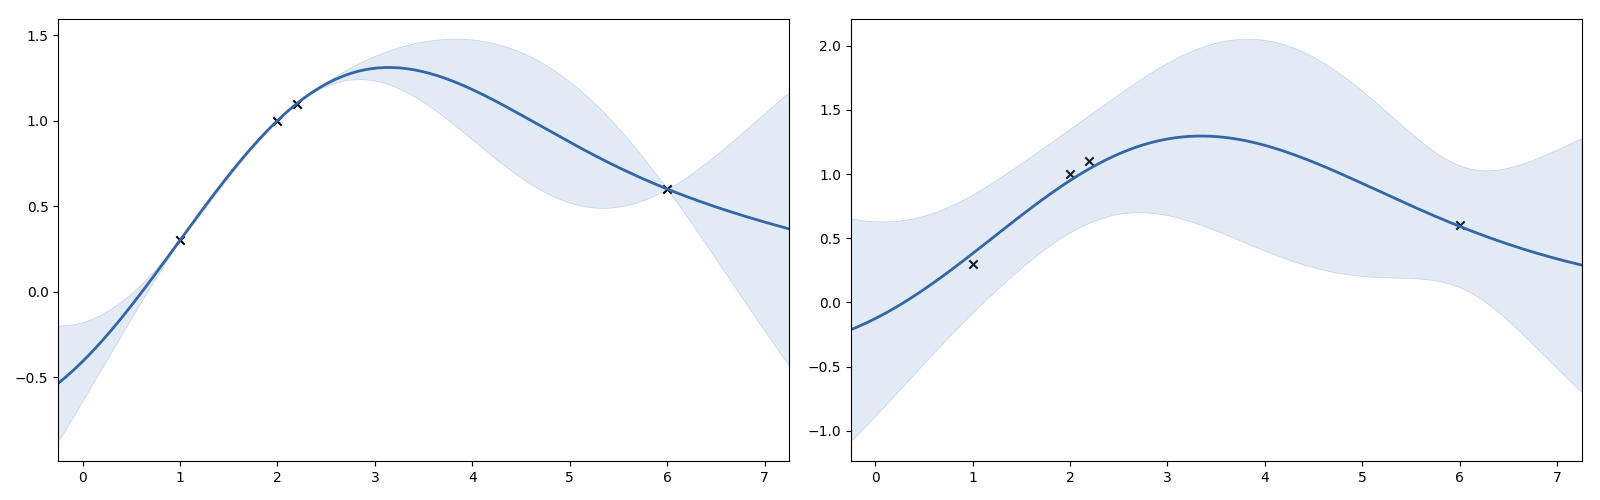
\includegraphics[width=1.0\textwidth]{images/gp-noise.png}
    \caption{GP regression without noise on the left, and with a constant
    amount of noise added on the right.}
	\label{figure:gp-noise}
  \end{center}
\end{figure}


\subsection{Kernels}
\label{section:kernels}

So far we have considered the covariance function $\kappa$ to be an arbitrary
positive-definite kernel. Even though in theory there are no restrictions on
what kernel we can choose, there are a few popular choices that are
commonly used.

A prototypical example is the squared exponential (SE) kernel, also called the
radial-basis function (RBF) kernel
$$
\kappa(x_1, x_2) = \sigma_k^2\exp\left\{ -\frac{1}{2 l} (x_1 - x_2)^2 \right\}.
$$
This kernel, among many others, falls under the category of stationary kernels.
A \newterm{stationary kernel} is a kernel which is shift-invariant, which means its
value does not depend on the absolute values of $x_1$ and $x_2$, but only on
their distance $d = |x_1 - x_2|$. We can thus write the kernel as
$$
\kappa(x_1, x_2) = \sigma_k^2\exp\left\{ -\frac{1}{2l} d^2 \right\}.
$$

The values $\sigma_k$ and $l$ are called the variance and the lengthscale, and control
the behavior of the kernel, where $\sigma_k$ changes the vertical scale of the
function, and $l$ changes the horizontal scale. Changing the lengthscale
essentially allows the kernel to re-normalize the data. If $\vx$ is a vector, we
can define a lengthscale parameter $l_i$ for each of the components. Such
component-specific lengthscale becomes very useful in the context of hyperparameters where each hyperparameter
can have quite a different scale, and the individual lengthscales per component
allow the kernel to capture the phenomenon.

\autoref{figure:gp-lengthscale} shows how the behavior of the kernel
changes based on the value of the lengthscale $l$. When the lengthscale
is set too low, the values of $y$ become essentially uncorrelated, leading to a
function with many spikes. On the other hand, a larger value for the lengthscale
yields a much smoother function.

\begin{figure}
  \begin{center}
    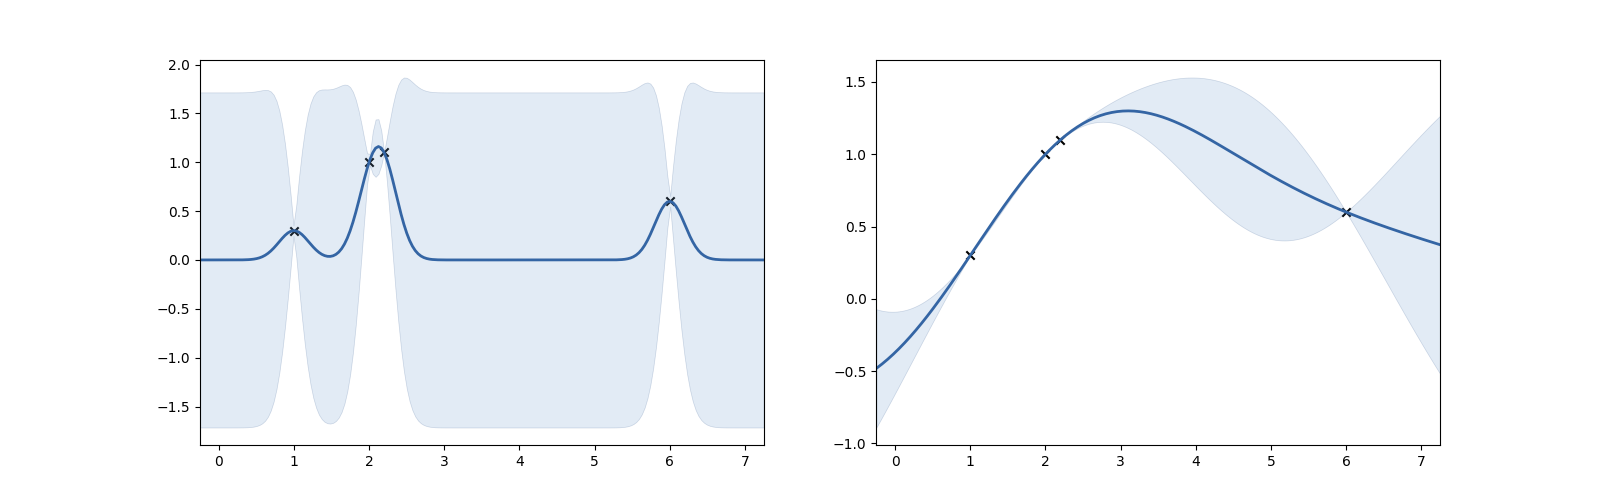
\includegraphics[width=1.0\textwidth]{images/gp-lengthscale.png}
    \caption{Lengthscale $l = 0.2$ on the left, and $l = 2$ on the right.}

    \label{figure:gp-lengthscale}
  \end{center}
\end{figure}

A popular kernel in the context of Bayesian optimization is the Mat\'ern kernel
$$
\kappa(d) = \frac{2^{1 - \nu}}{\Gamma(\nu)} \left( \frac{\sqrt{2\nu}d}{l} \right)^\nu K_\nu \left( \frac{\sqrt{2\nu}d}{l} \right)
$$
where $\nu$ and $l$ are the parameters and $K_\nu$ is a modified Bessel function \citep{williams2006gaussian}. In practice, we restrict ourselves to a half-integer variant of the Mat\'ern kernel, that is when $\nu = p + 1/2$, with $p$ being a non-negative integer. In this case the Mat\'ern kernel has a simplified form -- for example for $\nu = 5/2$, which is popular choice in ML, the covariance function simplifies to
$$
\kappa(d) = \left( 1 + \frac{\sqrt{5}d}{l} + \frac{5d^2}{3l^2} \right) \exp \left( - \frac{\sqrt{5}d}{l} \right),
$$
which ends causing the GP posterior to be $2$ times differentiable \citep{williams2006gaussian}, as compared to the RBF kernel shown above, which is infinitely differentiable. As a side note, the Mat\'ern kernel converges to the RBF kernel as $\nu \rightarrow \infty$.

In a general setting it could prove useful to examine many different kernel functions and use one that works best in a particular domain. However, in the case of Bayesian optimization, which should be sample-efficient, we consider only the kernels shown above, which have been shown to perform well in related work, especially the $5/2$ Mat\'ern kernel \citep{snoek2012practical}.

\subsection{Optimizing GP Hyperparameters}

\begin{figure}
	\begin{center}
		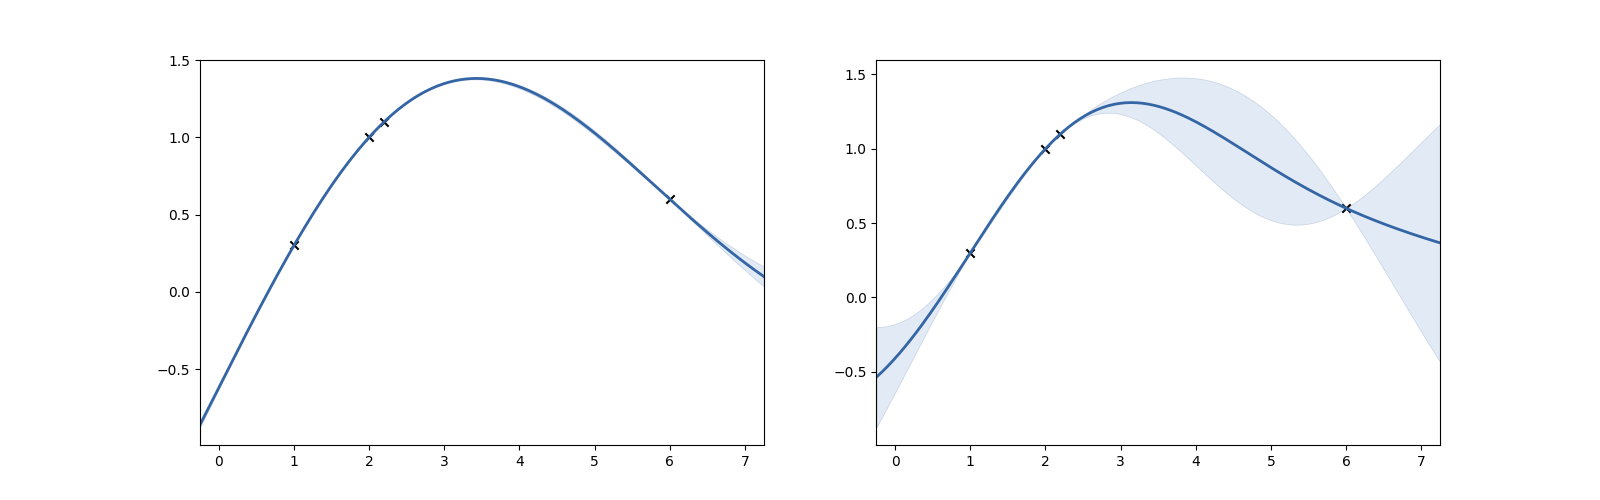
\includegraphics[width=1.0\textwidth]{images/gp-kernel-param-optimization.png}
		\caption{GP regression without optimizing kernel parameters on the left,
			and after optimizing using maximum likelihood on the right. Notice that
			the noise parameter is also optimized, as the regression model does not
			pass directly through the data points, but instead considers the small
			variation as due to noise.}
		\label{figure:gp-kernel-param-optimization}
	\end{center}
\end{figure}


So far we have considered the noise, variance and lengthscale parameters to be
fixed, but in this section we show how their value can be determined
automatically form the data using maximum likelihood estimation.

Since the GP is a probabilistic model, we can query it directly about the
likelihood of the data. Using the definition of a GP, we know that the
likelihood is a multivariate Gaussian, that is $p(\vy | \mX) =
\mathcal{N}(\vy | \mZero, \mK)$, giving us a log likelihood of
\begin{equation}
\log p(\vy | \mX) = -\frac{1}{2}\vy \mK^{-1}\vy - \frac{1}{2} \log \det \mK - \frac{N}{2} \log (2 \pi).
\label{eq:kernel-marginal-likelihood}
\end{equation}

We leave out the technical details (see \cite{williams2006gaussian} for
a detailed treatment) including the gradient of the marginal likelihood with respect to the
kernel parameters, because they do not provide any useful insights.

One important detail we want to stress out is that computing $K^{-1}$ takes
$\mathcal{O}(N^3)$, which puts a serious restriction on the size of the data we can fit
with exact GP regression. This does not concern us in the context of
hyperparameter optimization, where we prefer to stay within low hundreds of
evaluations anyway, but for other tasks it becomes a serious limitation.
Understandably, many workarounds for approximate inference were developed
\citep{williams2006gaussian}, which again we omit from this text, because they
are not relevant for hyperparameter optimization.

Implementing the kernel parameter optimization is simple in practice. One can
simply implement the marginal likelihood formula shown in
\autoref{eq:kernel-marginal-likelihood} and
use a package for automatic differentiation with an SGD or L-BFGS optimizer
to fit the parameters. Since the objective is non-linear, a common
practice \citep{gpy2014} is to optimize with multiple restarts.
\autoref{figure:gp-kernel-param-optimization} shows the effect of optimizing
kernel parameters using maximum likelihood. More details on optimizing the kernel
parameters can be found in \autoref{section:priors-on-kernel-params}.
